\documentclass[a4paper, 10pt]{article}

\usepackage[utf8]{inputenc}
\usepackage{fancyhdr}
\usepackage{pdfpages}
\usepackage{graphicx}
\usepackage{amsthm}
\pagestyle{fancy}
\setlength{\headheight}{24.0pt}

\clubpenalty10000
\widowpenalty10000
\displaywidowpenalty=10000

\rfoot{
	\begin{tabular}{r}
		Future User Interfaces\\
	\end{tabular}
}

\lhead{
	\begin{tabular}{l}
		SS 15\\
	\end{tabular}
}

\rhead{
	\begin{tabular}{l}
		Christoph Reinhart, Nicolas Spycher, Raphaël Thuor
	\end{tabular}
}

\begin{document}

	\title{Library application with gesture- and speech-based interface}
	\maketitle
	
	\begin{tabular}{rl}
		Christoph Reinhart  & christoph.reinhart@students.unibe.ch\\
		Raphaël Tuor  & raphael.tuor@gmail.com\\
		Nicolas Spycher & nicolas.spycher@students.unibe.ch
	\end{tabular}
	\newpage
	
	\tableofcontents
	\listoffigures
	\listoftables
	
	\newpage	
	\section{The application}
	
	\par{The idea behind the project, was to design and implement a Library Application which can hold the entire catalog of a Library and simplify the search and handling of the books. This would enable a library to display the whole collection of books, even if there isn't enough space on the shelves to display all of them. This system could be placed in the entryway of a library and give the customers the ability to browse the whole catalog even before entering the library itself.}
	\par{The application offers the user the ability to look up books and open them. The search function is programmed as a filter and displays all the available books if no filter is applied. The user is also able to bookmark the books he is interested in which then in a future version could be managed in some kind of user profile with a corresponding user login. Furthermore the applications provides the ability to mark a certain keyword in a opened book and use it as a search term. Other minor functionality includes jumping to a certain page and searching for keywords inside a book.}
	
	
	\section{The interfaces}
	
	\subsection{Gesture and speech}
	
	\par{The first interface is controlled with voice and gesture commands and is implemented using a Kinect device. The interface includes functionality that can be handled only with speech, only with gestures, with speech or gestures and some that can only be controlled using both inputs. Specific information about the commands follows in the next section}
	
	\subsection{Keyboard and mouse}
	
	\par{As a second interface we chose the traditional keyboard and mouse interface. This decision was made due to our main question which we wanted to be able to answer with this project. Our research question was, whether the use of a sophisticated interface can improve usability and productivity of the user or if on the other hand the keyboard and mouse interface is still a better way to go through information.}
	
	
	\section{Functionality}
	
	\par{This section gives an overview over the functionality of the application and positions the multimodal interactions according to the CASE and CARE models. The positioning is marked in brackets in the following format (CASE positioning / CARE positioning). In the future the speech and gesture interface is referred to as the 1st interface whereas the keyboard and mouse interface is referred to as the 2nd interface.}
	
	\subsection{Search}
	
	\subsubsection{1st interface}
	
	\par{If the user wants to search for a book he first has to say 'new search'. Then he can provide a keyword. This part of the interface is not multimodal. The found books are presented to the user with thumbnails of the book covers. To open a certain book the user has to move the mouse over the thumbnail with gestures and can then say the word 'open'  (Synergistic/Assignment). The book opens in the application itself.}
	
	\subsubsection{2nd interface}
	
	\par{The user can click in the search field and enter a keyword to search for certain books(Alternate/Assignment). For initiating the actual search he can ether press the search button or press the enter key. This would be Equivalence in the sense of the CARE model. To open a book the user clicks on the thumbnail with the mouse. (-/Assignment).}
	
	\subsection{Browsing book}
	
	\subsubsection{1st interface}
	
	\par{Once a book is open the user is presented with a couple of functionality. For example he can swipe horizontally to go from page to page (-/Complementarity). If he wants to jump to a certain page he can do so by saying 'jump to' and providing a page number by speech input (-/Assignment). The user is also able to search for a keyword in the book. He can do so by saying 'search for' and providing a keyword by speech input (-/Assignment). While in the search mode the user is able to go to the next occurrence of the word by saying the word 'next' or 'previous' (-/Equivalence).}
	\par{Furthermore the user can move the cursor over a word in the document with gestures and then say the word 'highlight' to highlight a certain word (Alternate/Assignment). After that he can search for this keyword by saying 'search for keyword' (-/Assignment).  }
	
	\subsubsection{2nd interface}
	
	\par{The same functionality is available for the keyboard and mouse interface. To go to the next or previous page or jump to a certain page the user has to use the predefined adobe acrobat reader controls of the application (-/Assignment). To scroll trough the document he can either use his mouse wheel or use the slider of the document viewer on the right side (-/Equivalence). If he wants to search for a word within the document he can either press ctrl+f or look for the functionality in the menu of the document viewer (-/Equivalence). To go to the next occurrence of the word he can use the mouse to click on the arrow buttons or use the keyboard arrow buttons (-/Equivalence).}
	\par{To use a word from the text as keyword the user has to copy the file into the search field and the initiate the search (Alternate/Assignment).}
	
	\subsection{Bookmark}
	
	\subsubsection{1st interface}
	
	\par{The user is also able to bookmark the books he likes to remember. To do so he first has to open a book as described before and then say the words bookmark or unbookmark if he wants to remove the book from his bookmarks (Alternate/Assignment). To get an overview over his bookmarks the user can say the word \"show bookmarks\" (-/Assignment).}
	
	\subsubsection{2nd interface}
	
	\par{For the keyboard and mouse interface this functionality is handled with three buttons for bookmarking, unbookmarking and show bookmarks. The user also hast to open a book first before he can use the buttons (Alternate/Assignment).}
	
	
	\section{Evaluation}
	
	\par{To evaluate both user interfaces and answer our research question we chose to do both qualitative and quantitative evaluation. Because of limited time and people we decided to do the evaluation within-group. The documents of the evaluation can be found in the appendix}
	
	\subsection{Research question}
	
	\par{Can the use of a sophisticated interface improve usability and productivity of the user or is the keyboard and mouse interface still a better way to go through information.}
	
	\subsection{Qualitative evaluation}
	
	\par{We used a questionnaire based on a template from Gary Perlman\footnote{http://garyperlman.com/quest/} . According to our general research goal we wanted to compare a multimodal interface with a traditional controlled interface. Therefore we asked the user after he interacted with both of these interfaces to rate them. The questionnaire was divided into four topics. 'Usefulness', 'Ease of use', 'Ease of learning' and 'Satisfaction'. The first part should review the general effectiveness of the two interfaces according to the judgment of the user. In the second part the user should describe how easy it was to interact with the system. In the third part the user should rate and compare the two ways of interaction, regarding to how quick he got accustomed with the possibilities of them. And the final part should reflect the general satisfaction of the user.}
	\par{The user was able to assign a scalar score from 1 to 7 (strongly disagree to strongly agree) to a bunch of closed questions. At the end a last question asked the user about his general preference for one or the other interface. To give the user the possibility to add some individual remarks about what he liked/disliked about each interface, we asked him to write down three positive and three negative aspects for each interface. Furthermore a general comment page allowed him to give even more feedback and his own opinion.}
	
	\subsection{Quantitative evaluation}
	
	\subsubsection{Evaluation setup}
	
	\par{As stated our set of users was rather small. Therefore we decided to do an evaluation within-group. Because our users where all within a range of age and intellect, where they already interacted a lot with mouse and keyboard, we first asked them to interact with the system by voice and gesture for two minutes without a specific task, to accustom them with voice and gesture interaction. Additionally we provided a set of instructions, which explained the functions of the application. We gave those instructions, because we wanted the application itself to be an independent variable. To diminish the learning effect, that occurs with a within-group setup, and the fact that the users were already accustomed to mouse and keyboard, we let them first interact with mouse and keyboard and then with gesture and voice.}
	\par{Each user received the following set of tasks, he or she should accomplish with both interfaces:}
	
	\begin{enumerate}
		\item Open the book 'A History of Mathematics'
		\item Search for the word 'Gutenberg' inside the book
		\item Go to page 10
		\item Bookmark this book.
		\item Bookmark the book 'First Six Books of the Elements of Euclid'
		\item Show all bookmarks
	\end{enumerate}
	
	\par{For later evaluation of the dependent variables we video-captured the screen and the user itself.}
	
	\subsubsection{Variables}
	
	\begin{itemize}
		\item \textbf{Independent variables:}
		\begin{itemize}
			\item Application
			\item Computer setup
			\item Subject type (average skilled computer user)
		\end{itemize}
		\item \textbf{Dependent variables:}
		\begin{itemize}
			\item Time to complete all tasks
			\item Number of steps (Number of mouse-clicks, number of mouse-drags, number of connected keys pressed\footnote{E.g. You need 4 keys to write the word 'five', we counted those pressed keys as 1.}, number of words spoken, number of gestures, number of arm movements).
			\item Number of recognition errors\footnote{E.g. The user said the correct word or made the correct gesture, but the system didn't recognize them correctly.}
	\end{itemize}
	\end{itemize}		
	
	\subsection{Results}
	
	\par{The evaluation was run on a group of six users, all within an age range of 20 to 60 years old. Before the evaluation they all knew how to use a computer and never had really used a Kinect or any gesture-and-voice interface previously. Our hypothesis was that keyboard and mouse interaction is more efficient than voice and gesture for the virtual library application.}
	
	\subsubsection{Qualitative results}
	
	\par{As we can see in figure \ref{fig:appreciation} on page \pageref{fig:appreciation}, the classical set of modalities mouse/keyboard was widely preferred by the users. This result is not surprising, as we will see it in the following of the results.}
	
	\begin{figure}[h]
		\centering
			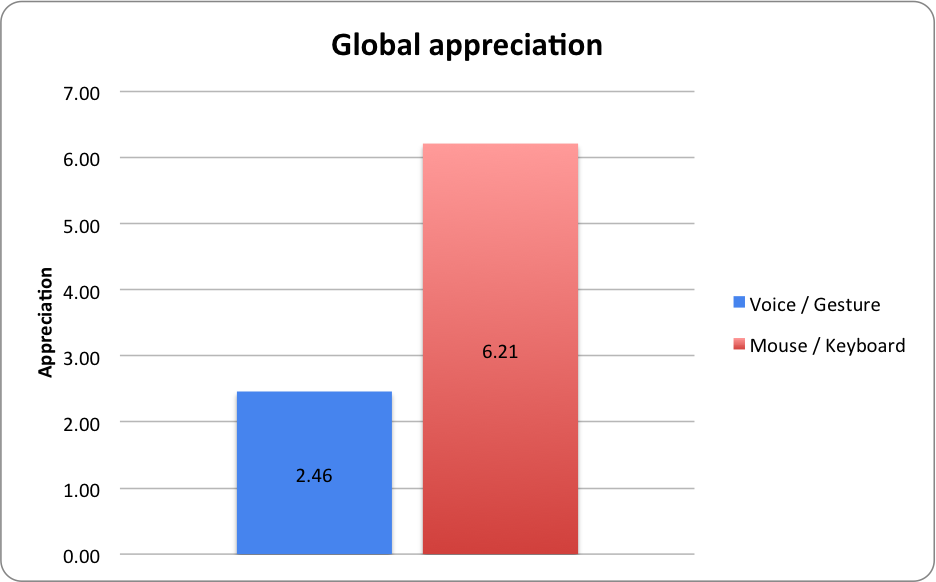
\includegraphics[scale=0.6]{graphs/globa_appreciation.png}
		\caption{Global appreciation}
		\label{fig:appreciation}
	\end{figure}
	
	\par{Figure \ref{fig:useful} and figure \ref{fig:easeofuse} on page \pageref{fig:useful}, show us that the users found the mouse/gesture a lot more effective to work with, and easier to interact with. We can attribute this result to the fact that users were more comfortable with an interface they already knew well and use everyday.}
	
	\begin{figure}[h]
		\centering
			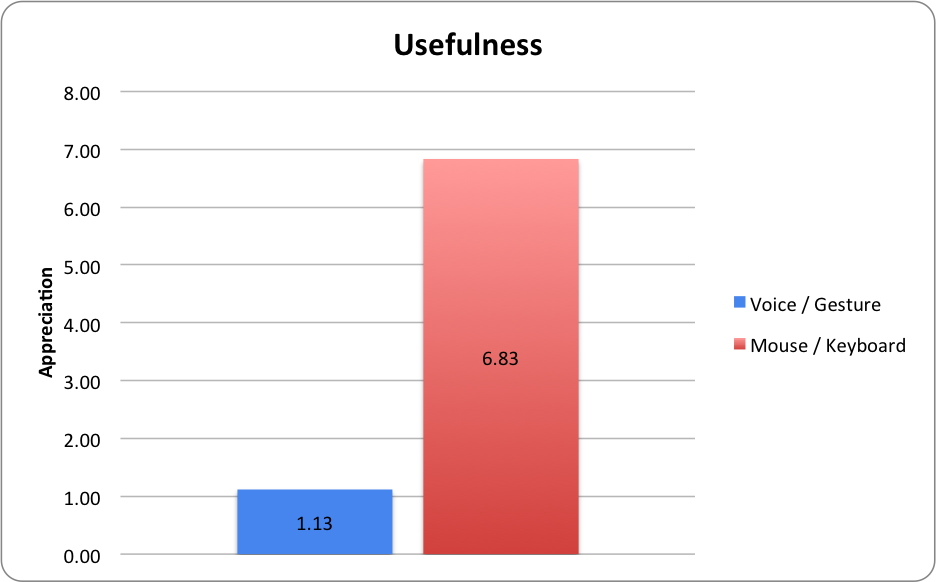
\includegraphics[scale=0.6]{graphs/usefulness.png}
		\caption{Usefulness}
		\label{fig:useful}
	\end{figure}
	
	\begin{figure}[h]
		\centering
			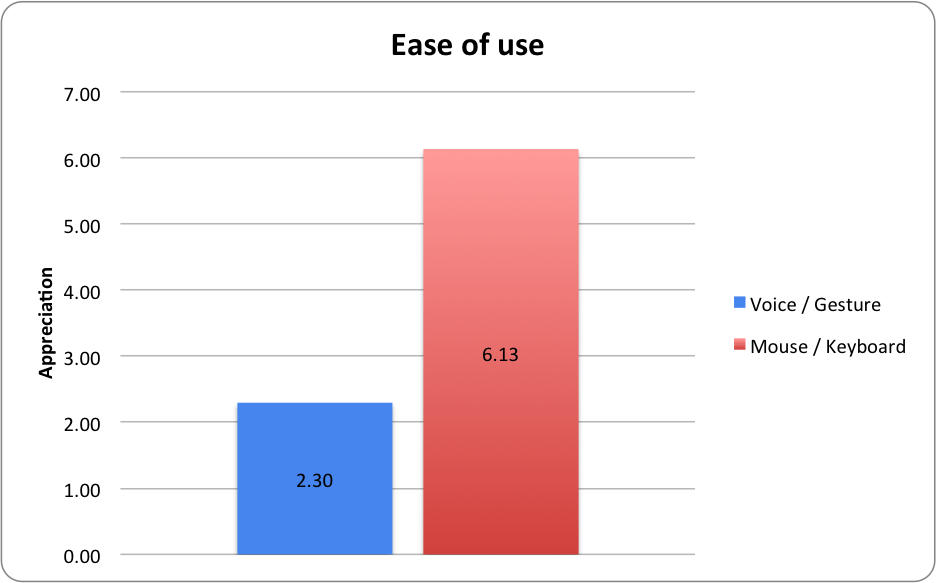
\includegraphics[scale=0.6]{graphs/ease_of_use.png}
		\caption{Ease of use}
		\label{fig:easeofuse}
	\end{figure}
	
	\par{Figure \ref{fig:easeoflearning} on page \pageref{fig:easeoflearning} shows an interesting contrast with the other qualitative results. While users preferred the mouse and keyboard interaction, they were confident in the fact that they would be able to learn to use the Virtual Library nearly as quickly with both interfaces. This result is encouraging, as it means that users do not feel too much difficulty in learning new modalities.}
	
	\begin{figure}[h]
		\centering
			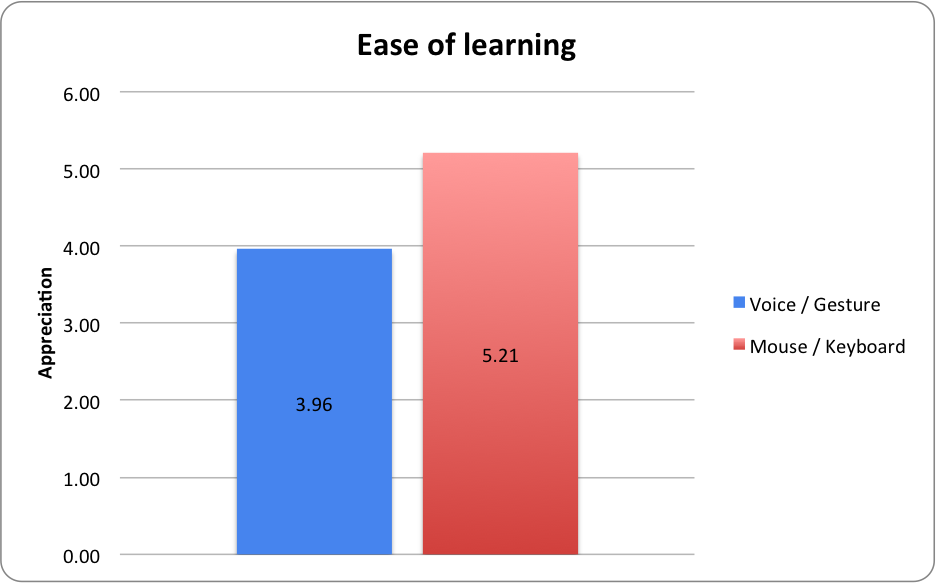
\includegraphics[scale=0.6]{graphs/ease_of_learning.png}
		\caption{Ease of learning}
		\label{fig:easeoflearning}
	\end{figure}
	
	\subsubsection{Quantitative results}	
	
	\par{Our hypothesis was that since users were already very familiar to the use of a mouse and a keyboard, they would be more efficient in the task they would be given. The results we obtained, visible in figure \ref{fig:completetask} on page \pageref{fig:completetask}, confirmed our prediction. Users completed the given task around three times faster with a mouse and a keyboard than with the voice and gesture commands.}
	\par{With the qualitative results in mind, we think that by giving the users more time to learn how to use the voice and gesture interface, the time difference between both interfaces would decrease significantly.}
	
	\begin{figure}[h]
		\centering
			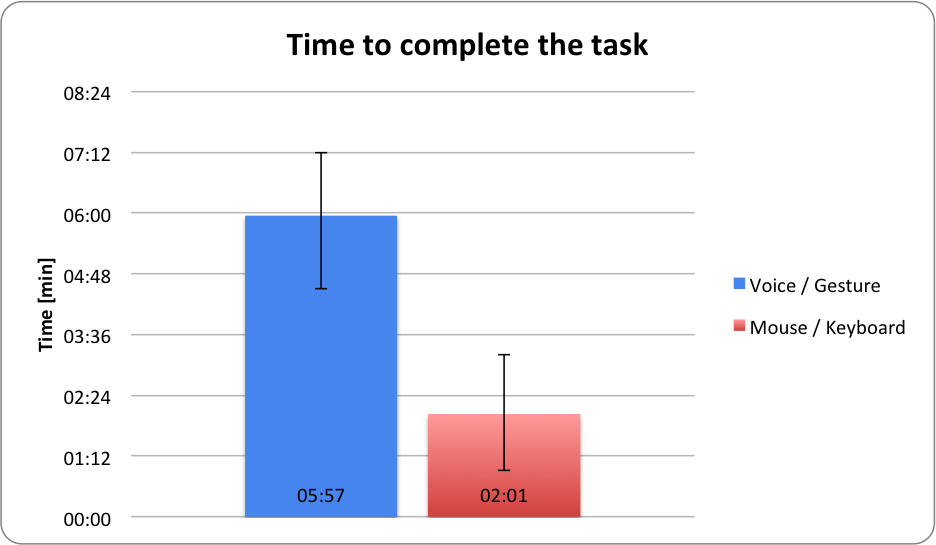
\includegraphics[scale=0.6]{graphs/time_to_complete_task.png}
		\caption{Time to complete task}
		\label{fig:completetask}
	\end{figure}
	
	\par{The steps required by the user to complete the given task were also measured. In figure \ref{fig:steptask} on page \pageref{fig:steptask} we can see that the voice and gesture interface required more steps. }
	
	\begin{figure}[h]
		\centering
			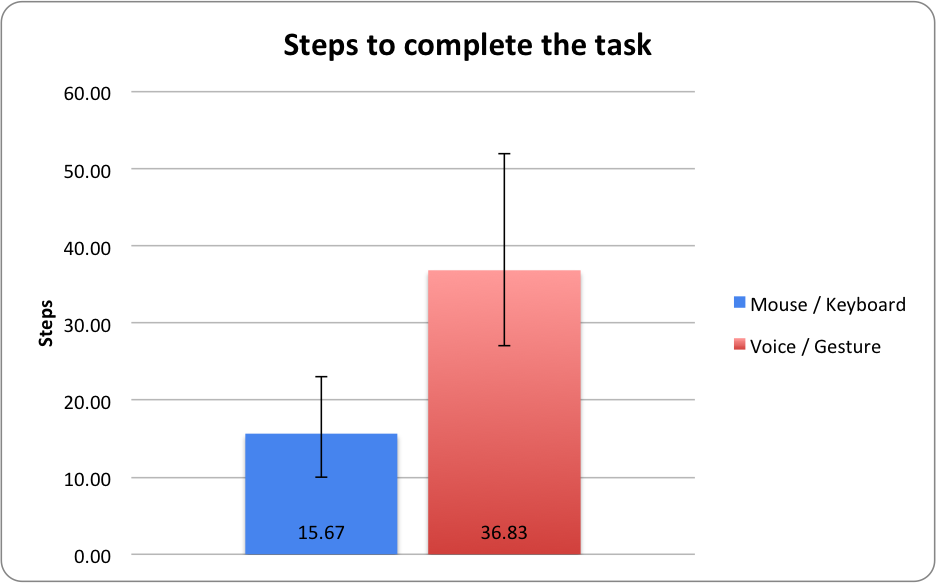
\includegraphics[scale=0.6]{graphs/steps_to_complete_task.png}
		\caption{Steps to complete task}
		\label{fig:steptask}
	\end{figure}
	
	\par{According to us, this is mainly due to the recognition errors that occurred with the speech and gesture recognition. As we can see in table \ref{tab:errors} on page \pageref{tab:errors}, on average 20.5 errors occurred for each user while using voice and gesture, and only 1 occurred with the mouse and keyboard interface.}
	\par{Moreover, among these 20.5 errors, about 60\% were due to the system itself (e.g. not understanding a word, missing track of the hand). If the ergonomics of the virtual library were improved, most of these errors would probably not occur. The remaining 8 errors can be imputed to the fact that the users were not familiar with voice and gesture systems, and did not know very well how to behave with it.}
	
	\begin{table}
	\centering
		\begin{tabular}{| l | p{2.4cm} | p{2.4cm} | p{2.4cm} |}
			\hline
			\textbf{Type of interface} & Users errors (average) & Recognition errors (average) & Total (average)\\
			\hline
			Mouse and keyboard & 1 & 0 & 1 \\
			\hline
			Voice and gesture & 8 & 12.5 & 20.5 \\
			\hline
		\end{tabular}
		\caption{Errors}
		\label{tab:errors}
	\end{table}
	
	\par{In conclusion of these results, we can say that our hypotheses revealed to be true: keyboard and mouse interaction is more efficient that voice and gesture for a virtual library application. One of the possible explanations is that the mouse and keyboard are widely used since decades, as voice and gesture systems just start to be adopted by consumers (e.g. Google Now, Apple’s Siri, Samsung TVs). The overall efficiency of gesture and voice commands would certainly increase if its ergonomics were improved accordingly to further user centered design evaluations (by giving the user more feedback, e.g.), and if more time was given to the users to get familiar with the voice and gesture system.}
	
	\section{Conclusion}
	
	\par{According to the results of our evaluation, we should say that mouse and keyboard interaction is more efficient, useful, satisfying and precise than a multimodal way of interaction, as represented by voice and gesture interaction in our system.}
	\par{But the low scoring of the voice/gesture-input can be traced back to several circumstances. First of all: the efficiency and usefulness of a modality is strongly dependent on the task it is used for, the feedback, which is given to the user and the environment it is used in. }
	\par{Our main mistake was to try to use a voice-gesture-interaction with a classical GUI-interface. The user had to stand a certain distance to get recognized by the Kinect. It was impossible to read the small GUI-Elements from such a distance, therefore he had to get nearer and therefore his gestures could no longer be interpreted by the system. It would have been more successful to use also more channels for the output (e.g. synthetic speech).}
	\par{Further problems were technical challenges. The visual tracking of the Kinect did not work if the user moved his limbs too quickly. Therefore he had to move slowly and because of that the efficiency of the system was reduced a lot.}
	\par{A positive aspect of our gesture-voice-interface, which we could observe during evaluation, was the flexibility of redundant or equivalent modalities. User often switched from gesture to voice and vice versa, if the Kinect didn't interpret the input correctly. Redundant or equivalent modalities are therefore a really useful instrument for error correction. We could also observe how users changed modalities if the situation asked for it. E. g. a user was interacting with the system through gesture, if his hands were occupied because he had to read the instructions, he immediately changed to voice-interaction.}
	\par{As a final conclusion we can state, that multimodal interfaces can be more efficient, faster, flexible and less erroneous, but only if you implement them thoughtfully, with according feedback and with enough sensor-precision.}
	
	
	
	
	
	
	
	\newpage
	\appendix
	
	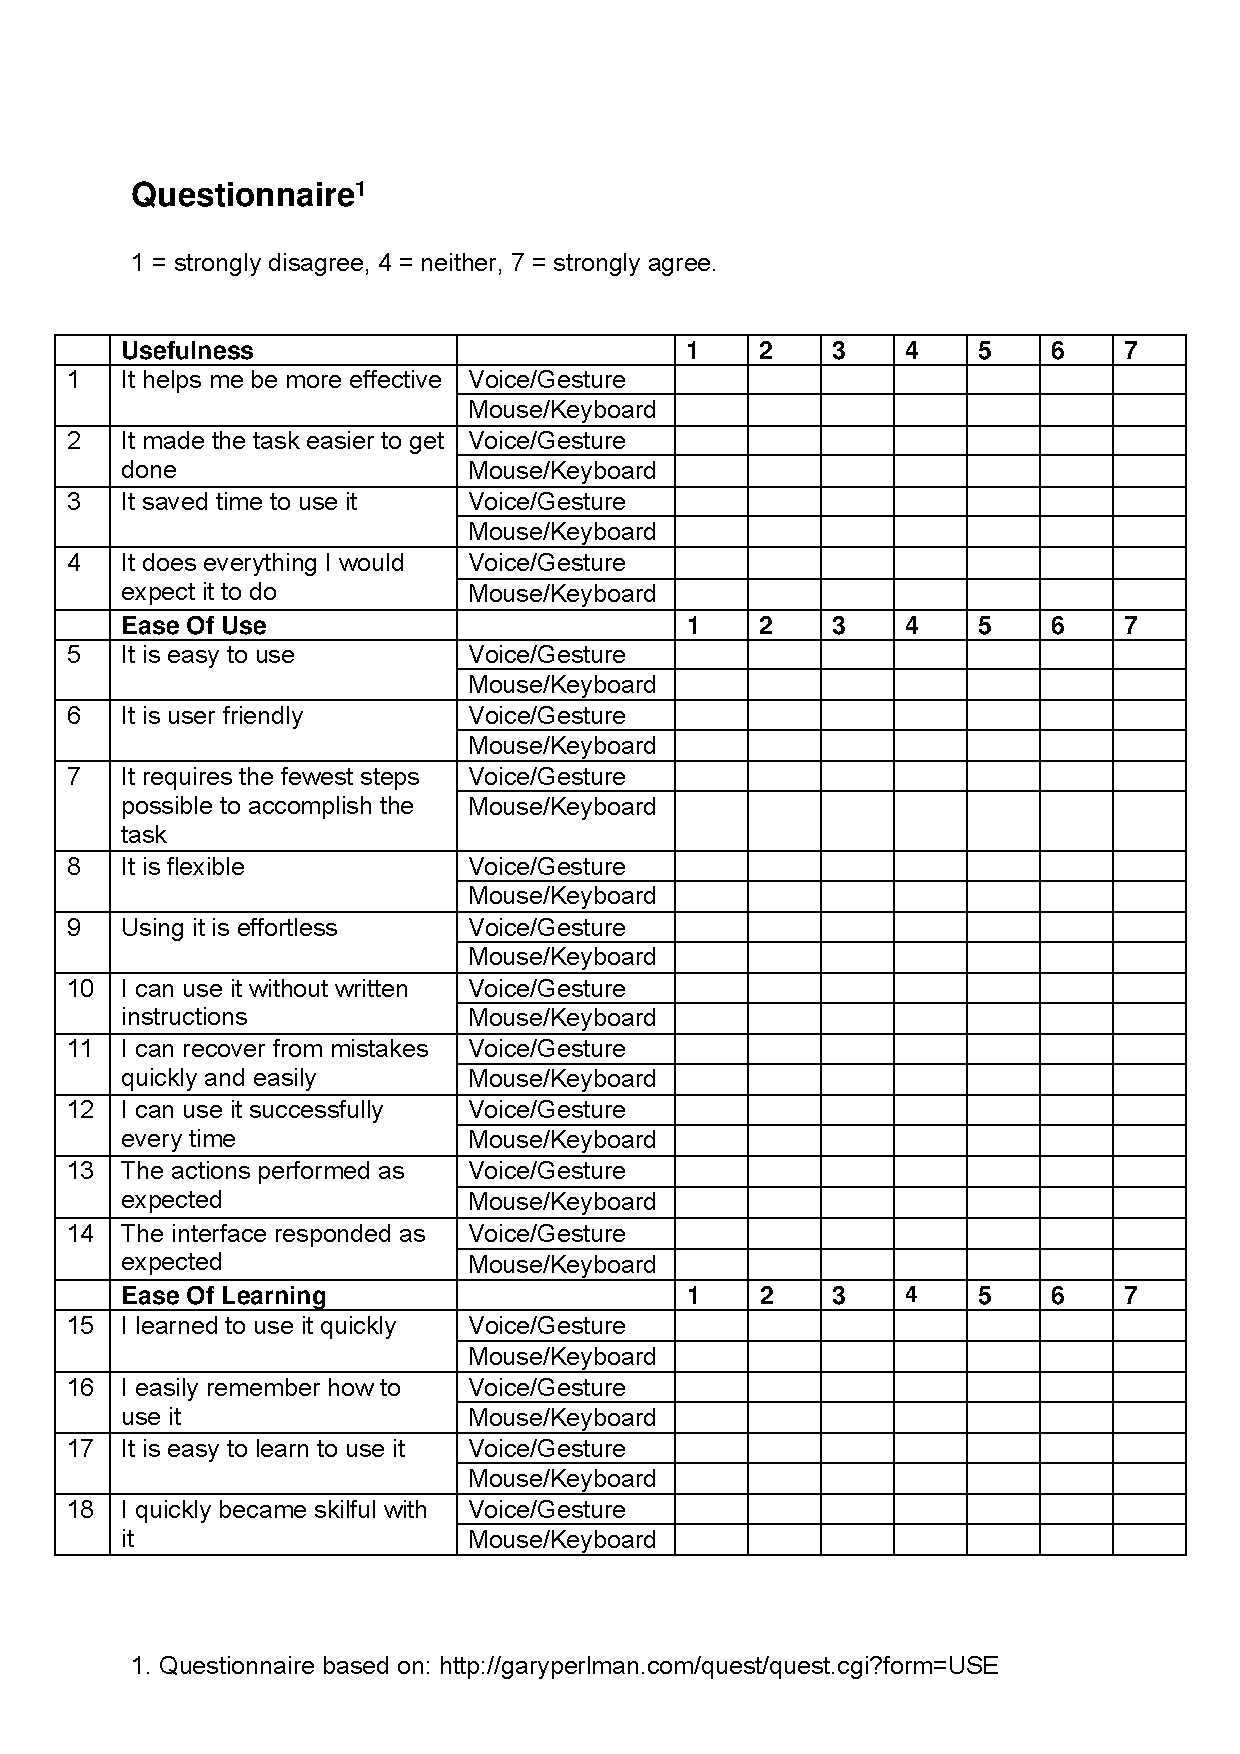
\includepdf[scale=0.8, page=1, pagecommand=\section{Questionnaire}]{questionnaire.pdf}
	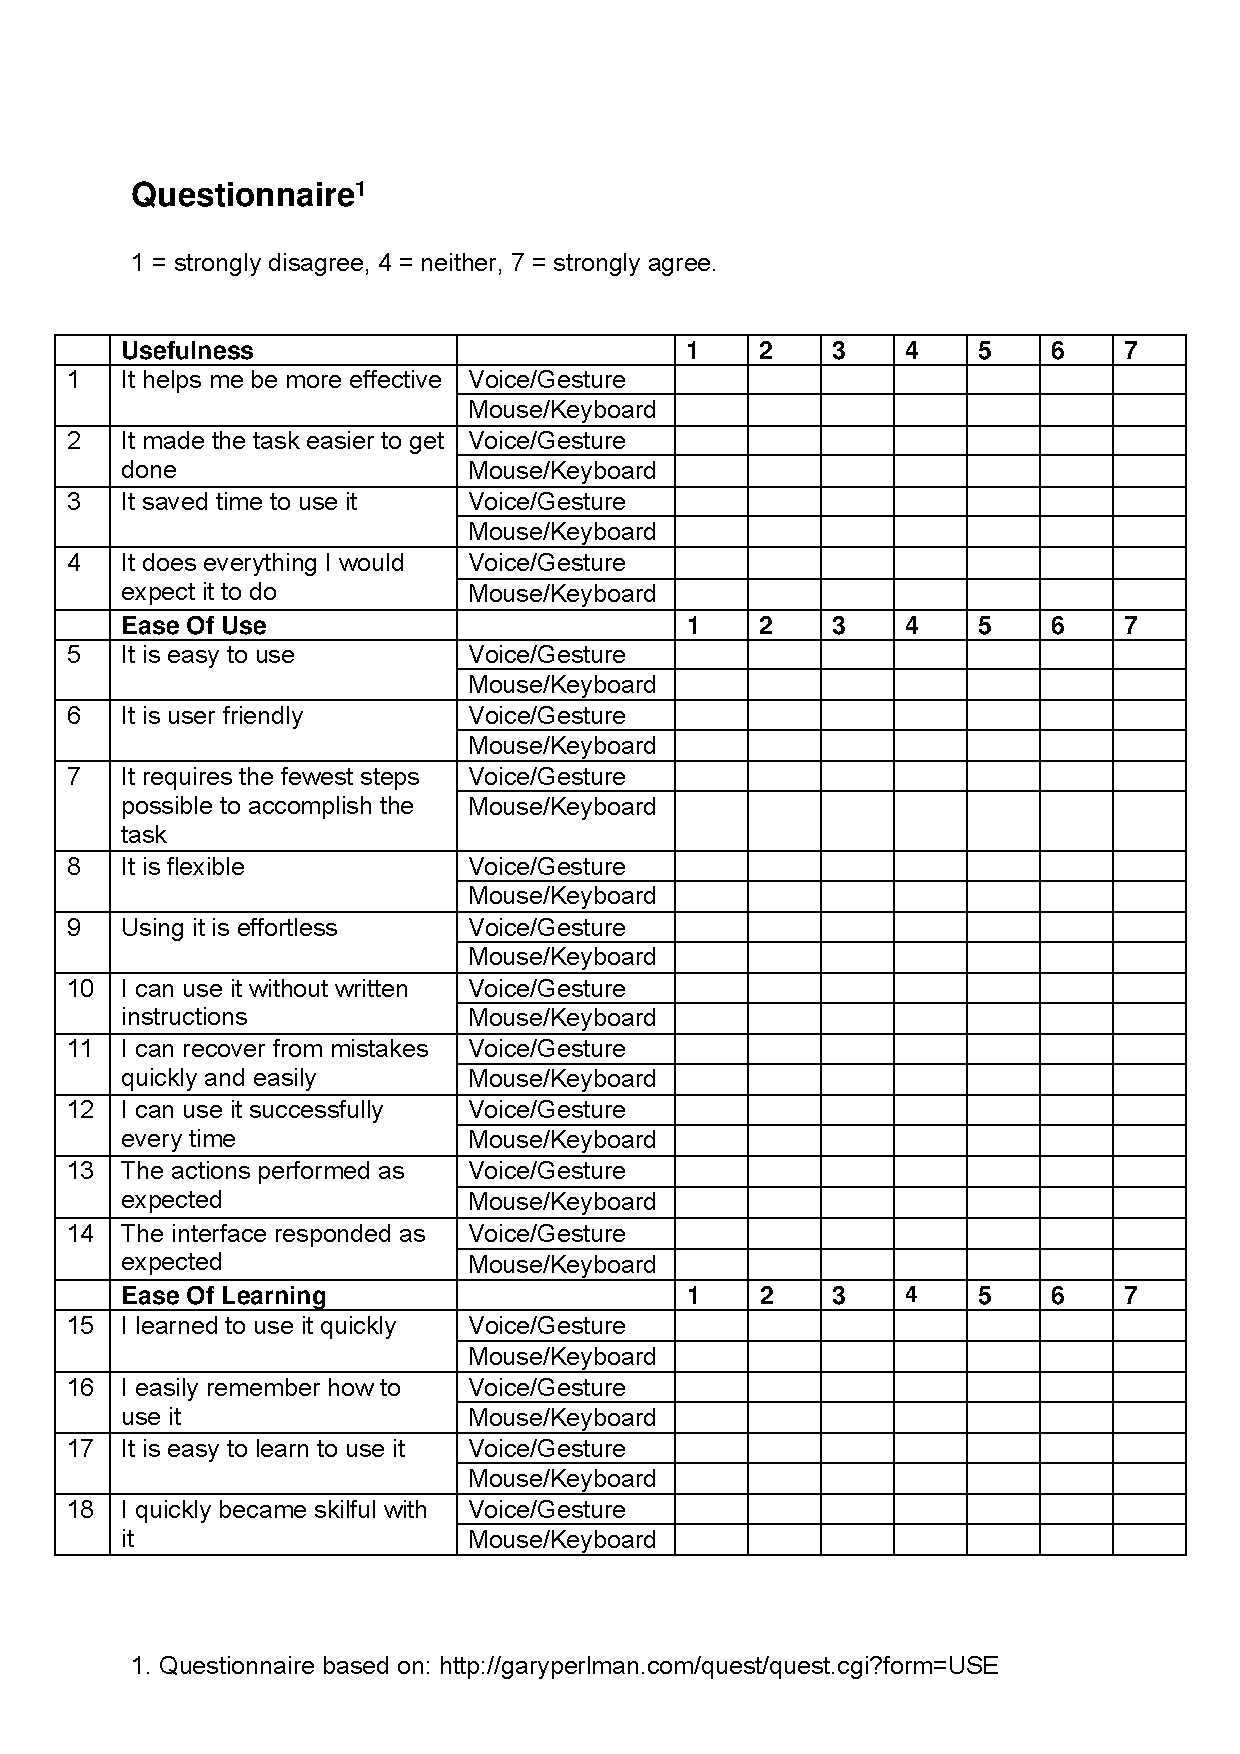
\includepdf[scale=0.8, page=2-, pagecommand={}]{questionnaire.pdf}
	
	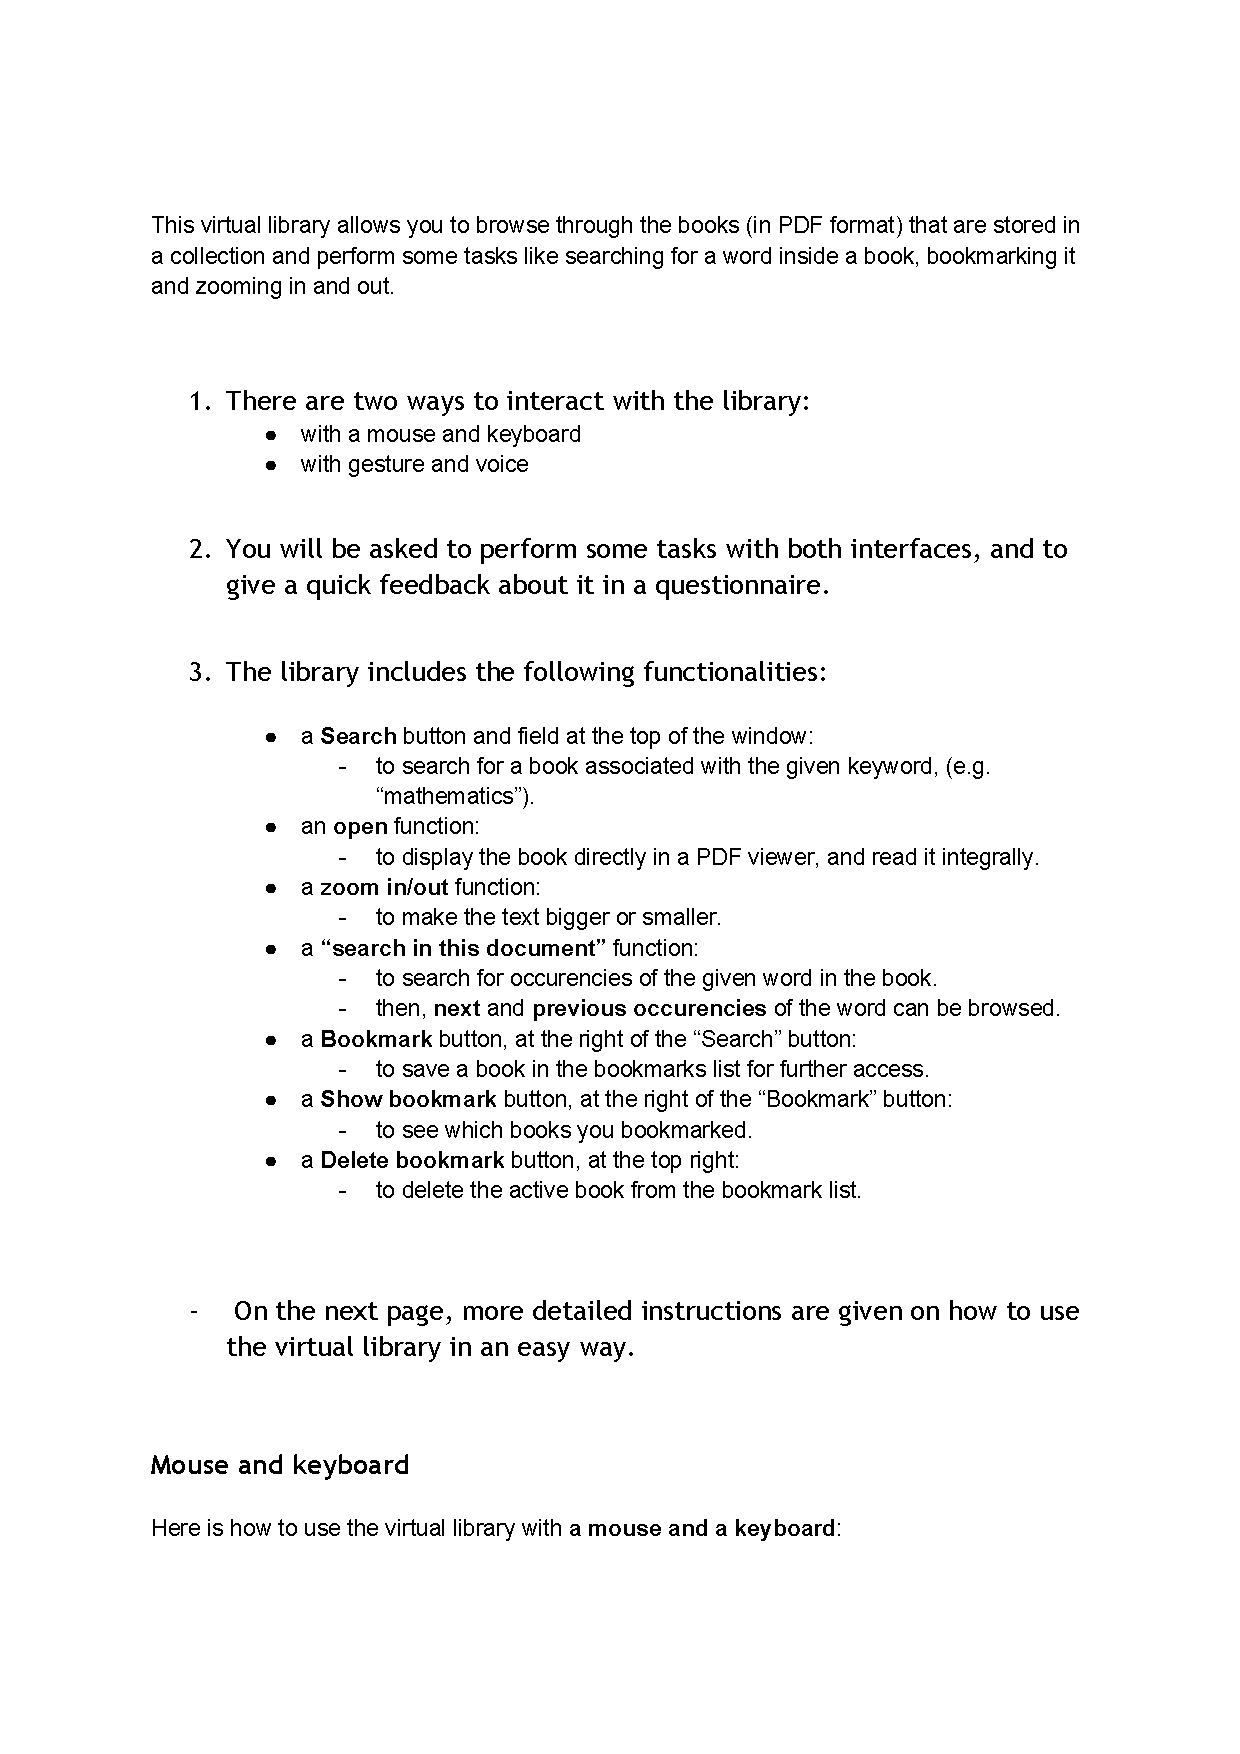
\includepdf[scale=0.8, page=1, pagecommand=\section{User instructions}]{user_instructions.pdf}
	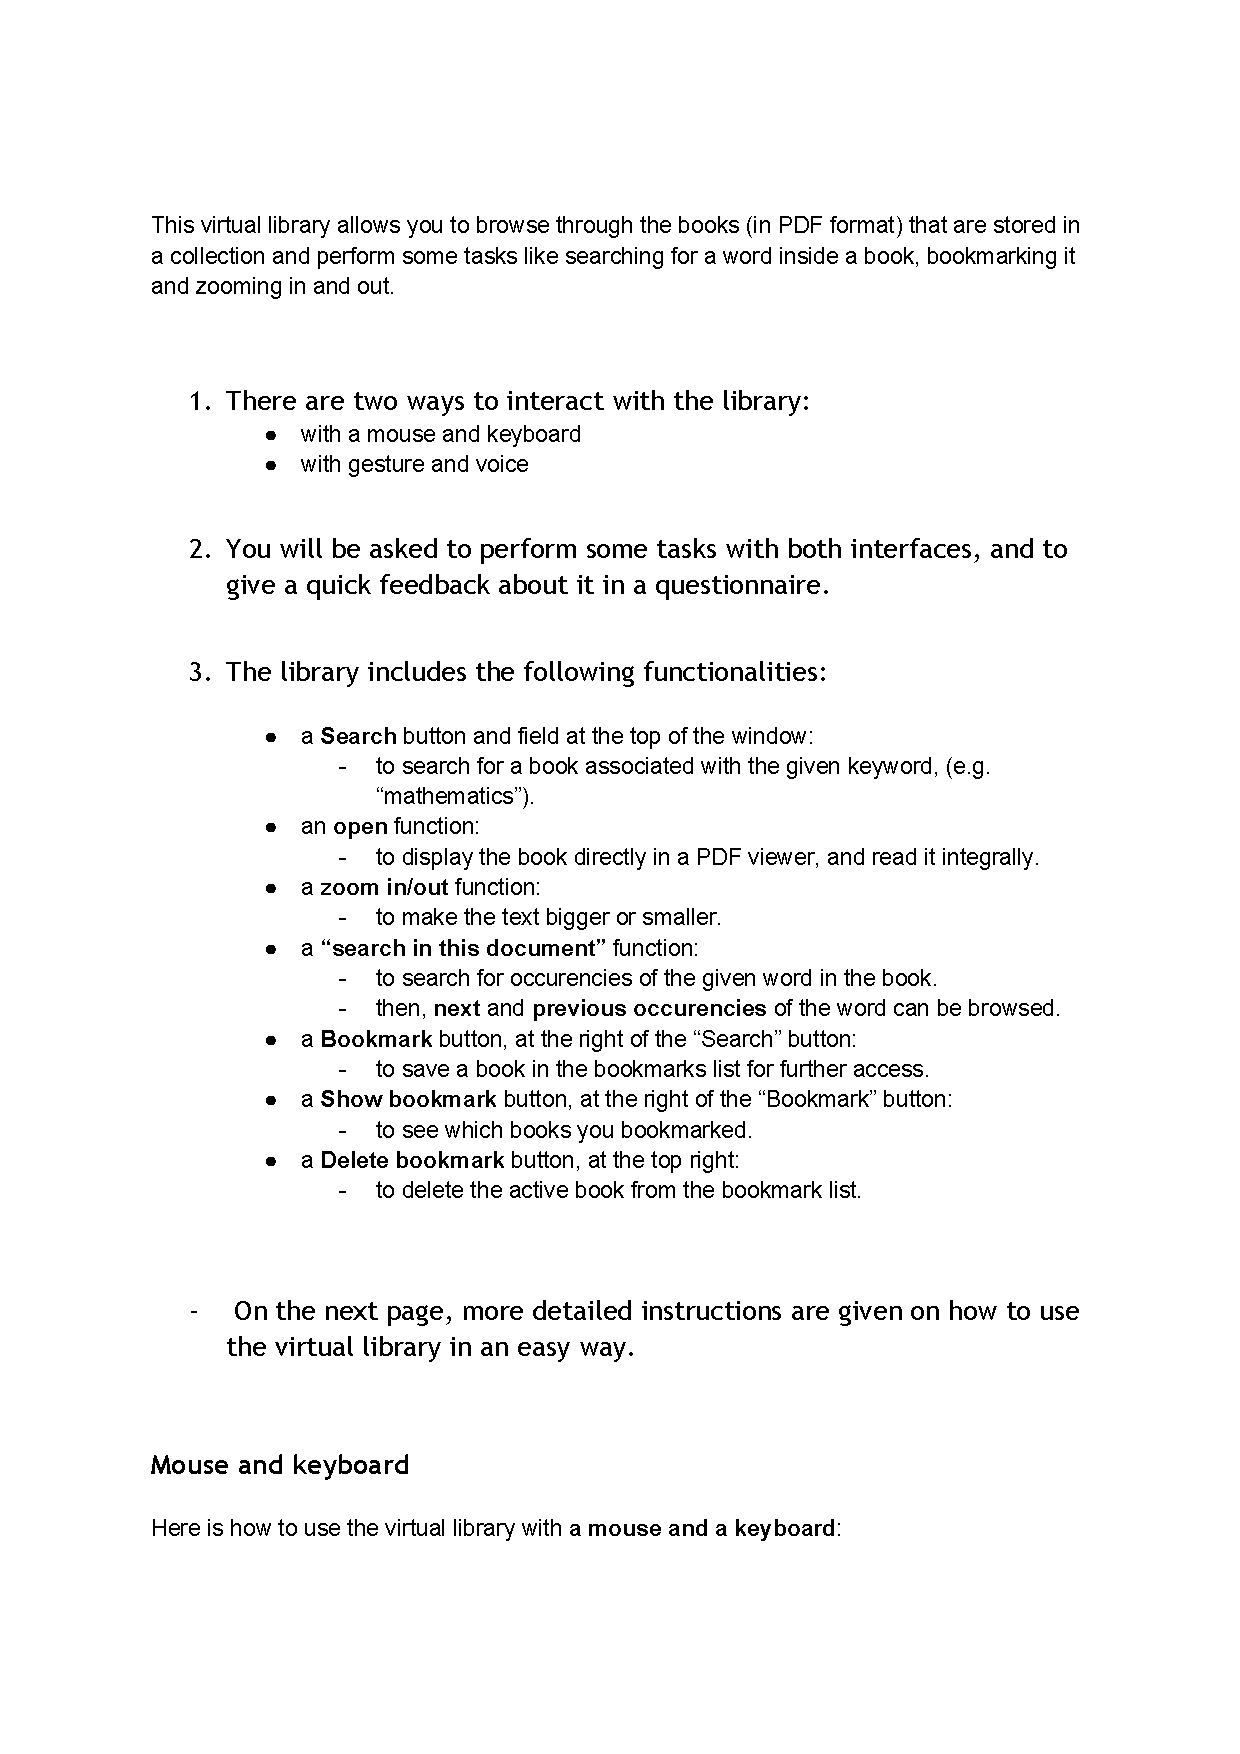
\includepdf[scale=0.8, page=2-, pagecommand={}]{user_instructions.pdf}
	
	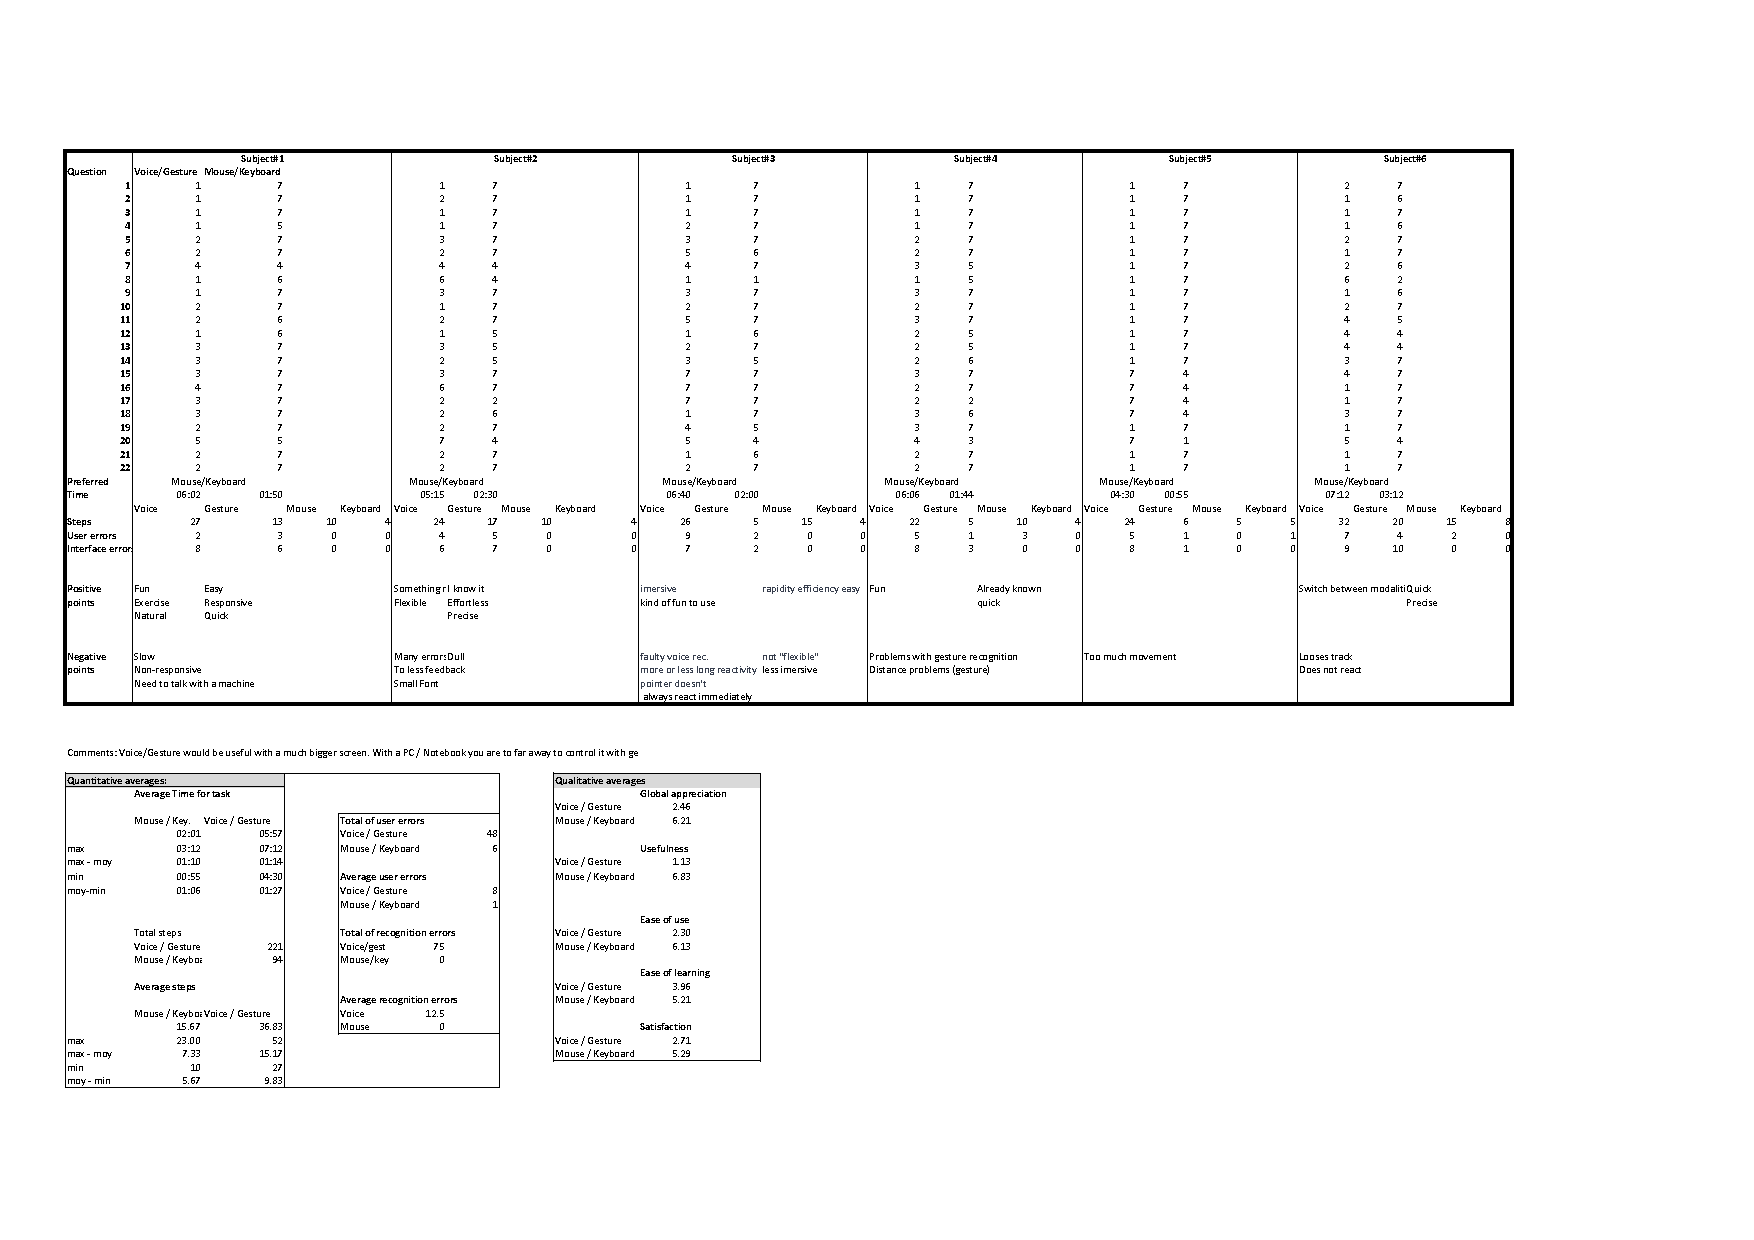
\includepdf[scale=0.85, angle=90, page=1, pagecommand=\section{Evaluation results}]{evaluation_results.pdf}
	
	
	
	
	

\end{document}
